\section*{Capítulo 02: Homem contratual}

Alguns dos temas resenhados deste capítulo já foram tratados na resenha entregue anteriormente. Por conta disso, será feita uma resenha mais direta, retomando a conexão entre os conceitos e pontuando as diferenças com o capítulo de Farina el all (1997). Dito isso, neste capítulo, Williamson analisa as diferentes abordagens dos contratos no que diz respeito à: (1) hipótese comportamental; (2) atributos das transações e; (3) o grau as disputas são resolvidas internamente ou esfera jurídica. Os dois primeiros temas são tratados neste capítulo enquanto o capítulo seguinte avança no terceiro.

\subsection*{Hipóteses comportamentais}

De modo geral, economistas partem de hipóteses comportamentais por conveniência e simplificação enquanto a ECT parte da racionalidade limitada e comportamento oportunista.

\subsubsection*{Racionalidade}

\begin{description}
	\item[Maximizadora:] Racionalidade forte em que todos os custos relevantes são identificados. Instituições dão lugar à funções-objetivo.
	\item[Limitada:] Racionalidade \textbf{intencional} e limitada em que a captura e processamento de informação são escassos. Como consequência, se faz necessário estudar organizações que vão além dos mercados.
	\item[Orgânica:] Presente na literatura austríaca e neo-Schumpeteriana. A primeira enfatiza processos gerais e instituições ``não planejadas''. A segunda vertente trata de processos evolucionários dentro e ente firmas
\end{description}


\subsubsection*{Autointeresse}

Os diferentes tipos de comportamento autocentrado são

\begin{description}
	\item[Oportunismo:] Refere-se à distorção das informações, especialmente para esforços calculados para enganar, distorcer disfarces, ofuscar ou confundir. Em linhas gerais, transações que estão sujeitas ao oportunismo \textit{ex post} se beneficiarão de salvaguardas elaboradas \textit{ex ante}. Além disso, oportunismo está associado com \textbf{incerteza} das transações econômicas
	\item[Oportunismo simples] Já descrito em outra resenha
	\item[Obediência] Já descrito em outra resenha
\end{description}


\subsubsection*{Comparações}

A tabela abaixo permite uma comparação entre as diferentes abordagens de acordo com as hipóteses comportamentais. Uma vez que é autoexplicativa, não será analisada em maiores detalhes e serão elencados pontos referentes à ECT e não às demais:

\begin{figure}[H]
	\centering
	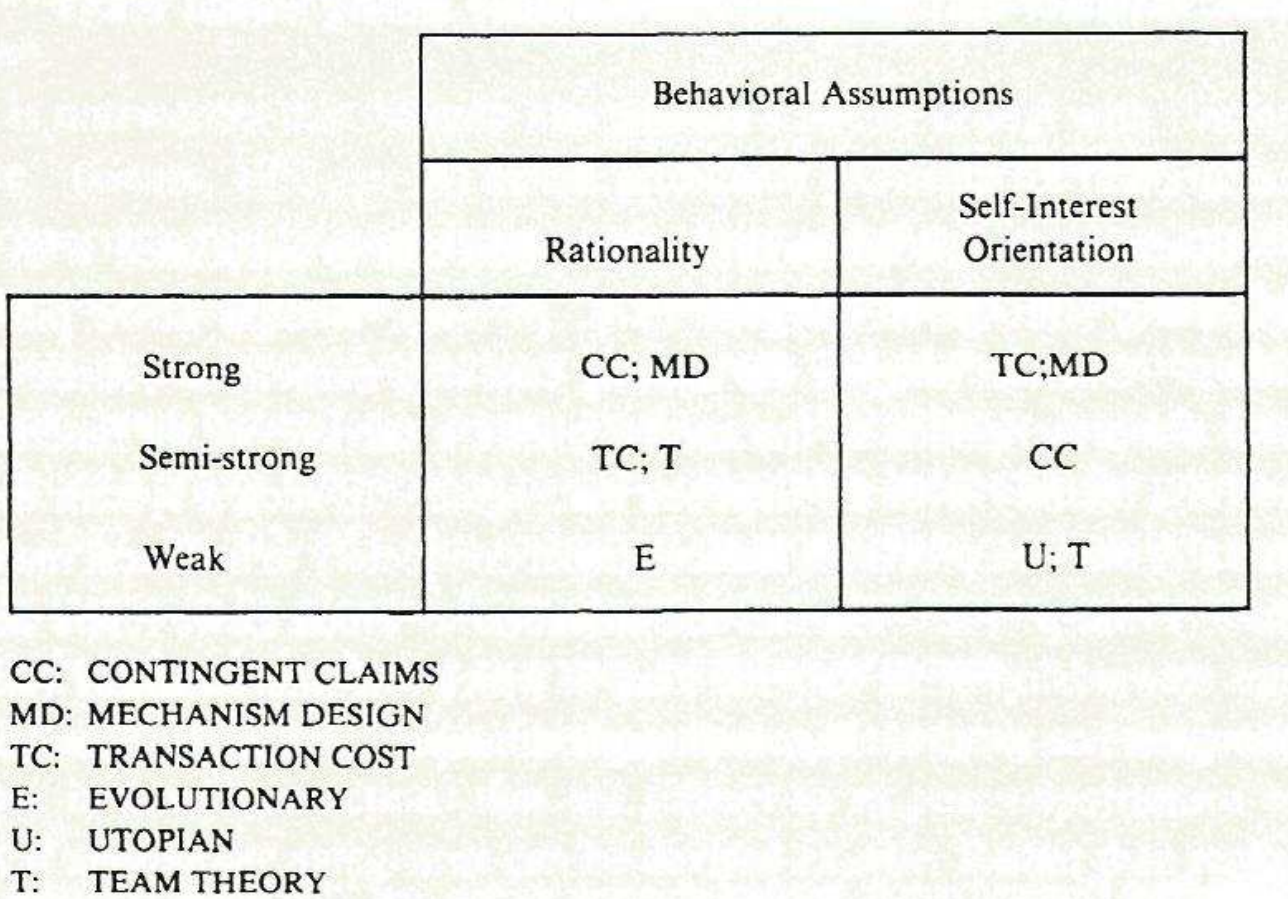
\includegraphics[width=0.7\linewidth]{screenshot004}
	\caption{Hipóteses comportamentais de abordagens organizacionais alternativas}
	\label{fig:screenshot004}
\end{figure}

\subsection*{Dimensões}

\subsubsection*{Especificidade dos ativos}

Williamson destaca que apesar da especificidade dos ativos já ter sido apresentada em trabalhos anteriores, eram considerados insignificantes e, por conta disso, eram desconsiderados. Argumenta que a especificidade dos ativos surgem em um contexto \textbf{intertemporal}. Podem ser caracterizados como: são ativos que não podem ser empregados em funções as quais não foram designados sem perdas significativas de valor, ou ainda, seu valor se reduz se a \textbf{transação} a qual lhe é específico é interrompida. Ao considerar a especificidade dos ativos, surgem \textit{trade-offs} que precisam ser considerados que, por sua vez, são particulares da estrutural de governança. Para esclarecer algumas diferentes entre conceitos contratuais e contábeis, o autor apresenta o esquema abaixo em que diferencia custos associados à especificidade dos ativos ($v$) dos custos fixos ($F$) e variáveis ($V$):

\begin{figure}[H]
	\centering
	\caption{Distinção dos custos}
	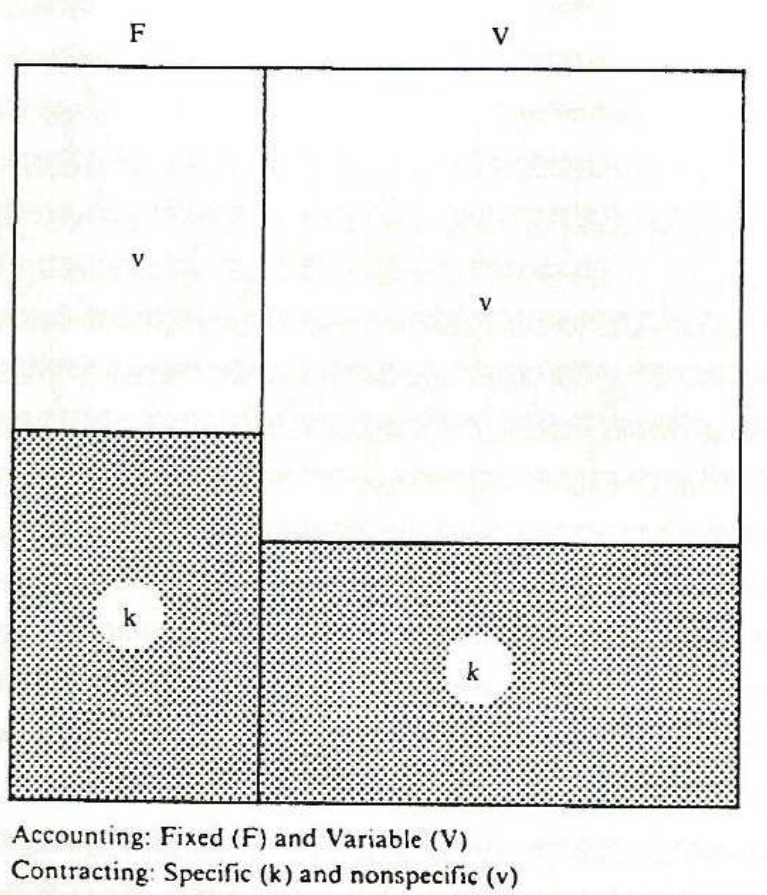
\includegraphics[width=0.7\linewidth]{screenshot005}
	\label{fig:screenshot005}
\end{figure}

Em seguida, o autor pontua que a \textbf{transformação fundamenta} decorre da especificidade dos ativos que, por sua vez, podem ser distinguidos em:
\begin{itemize}
	\item especificidade física
	\item especificidade humana
	\item ativos dedicados
\end{itemize}
Além disso, destaca:
\begin{itemize}
	\item Especificidade dos ativos diz respeito à investimento duráveis associados à transações particulares, em que o custo de oportunidade do investimento é menor que o uso alternativo dos recursos
	\item Identidade das partes é relevante para a continuidade da transação
	\item Salvaguardas organizacionais e contratuais surgem para dar conta deste tipo de transação
	\item A importância da especificidade dos ativos deve ser considerada em conjunto com a racionalidade limitada e comportamento oportunista
	\item A análise acentuada de formas organizacionais convencionais se deve à desconsideração da especificidade  dos ativos
\end{itemize}

\subsubsection*{Incerteza}

Além das discussões sobre incerteza, o autor destaca que quanto maior o grau de incerteza, mais impositivo é a especificidade dos ativos.

\subsubsection*{Frequência}

Resumidamente, estruturas de governança especializadas são mais sensíveis à transações específicas do que estruturas de governança de propósito mais geral. No entanto, estruturas de governança específicas são custosas e o que deve ser avaliado é quando estes custos são justificados. Em linhas gerais, os benefícios de estruturas de governança específicas são maiores quão mais frequente a transação é quanto mais específicos são os ativos que ela diz respeito. Desse modo, o objetivo da estrutura de governança é reduzir os custos de transformação e de transação, não apenas um deles.

\subsection*{Transformação fundamental}

Como destacado anteriormente, a ECT reconhece a importância do estabelecimento contratual \textit{ex ante}, mas dá maior ênfase à execução (relação contratual\textit{ex post}). Além disso, pontua que relações contratuais mais numerosas não implicam necessariamente em maior eficiência, ou melhor, que tais relações contratuais irão prevalecer. Em resumo, a identidade contratual é relevante para a continuidade das relações entre as partes. Nesses termos, define a transformação fundamental nos seguintes termos:

\begin{description}
	\item[Definição:] É definido como a transformação de um conjunto numeroso de contratantes em uma relação bilateral
\end{description}
Argumenta que esta transformação tem implicações importantes como descrito abaixo (p.~63, grifos adicionados):

\begin{quotation}
	\textit{
	Joined as they are in a condition of \textbf{bilateral monopoly}, both buyerand seller are strategically situated to bargain over the disposition of any incremental gain whenever a proposal to adapt is made by the other party. [...]
	Efficient adaptations that would otherwise be made thus result in costly haggling or even go unmentioned, lest the gains be dissipated by costly	subgoal pursuit. Governancestructures that attentuate opportunism and otherwise infuse confidence are evidently needed.
	}
\end{quotation}